\subsection*{Связи агентов -- добавление, удаление, список, количество}
\addcontentsline{toc}{subsection}{Связи агентов -- добавление, удаление, список, количество}

\textbf{Задание:}\\
\begin{enumerate}[topsep=0pt,itemsep=-1ex,partopsep=1ex,parsep=1ex]
	\item Создать популяцию агентов. Отобразить агенты и их связи. Для визуализации агентов
	использовать круг и текст с номером агента в популяции.
	\item Предусмотреть:
	\begin{itemize}[topsep=0pt,itemsep=-1ex,partopsep=1ex,parsep=1ex]
		\item добавление в популяцию нового агента отображение обновленной популяции;
		\item добавление/удаление связи между случайными агентами;
		\item добавление/удаление связи между агентами с заданными номерами. Номера задавать с помощью выпадающих списков.
	\end{itemize}
	\item Выделить цветом агента с максимальным количеством связей, вывести количество связей.
	\item Выделить цветом агентов, связанных с заданным.
	\item Предусмотреть удаление сделанных цветом отметок.\\
\end{enumerate}

\textbf{Решение:}\\
Для начала необходимо создать популяцию агентов. У агентов будет их порядковый номер, текстовая метка которая отражает данную информацию и текстовая метка, которая показывает сколько других агентов связано с текущим. (Рисунок \ref{fig:agents1})
\begin{figure}[h]
	\centering 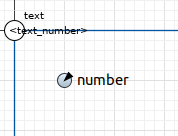
\includegraphics[scale=0.4]{agents1}
	\caption{Параметры популяции}
	\label{fig:agents1}
\end{figure}

Добавление новых агентов осуществляется по кнопке, также в данной кнопке осуществляется добавление нового агента в ComboBox. (Рисунок \ref{fig:agents2})
\begin{figure}[h]
	\centering 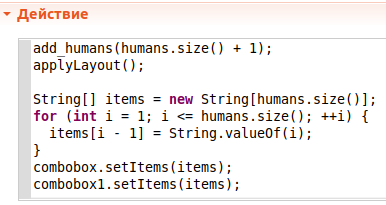
\includegraphics[scale=0.35]{agents2}
	\caption{Реализация логики добавления нового агента}
	\label{fig:agents2}
\end{figure}

\newpage

В самом начале при запуске модели осуществляется добавление всех сгенерированных агентов в ComboBox. (Рисунок \ref{fig:agents3})
\begin{figure}[h]
	\centering 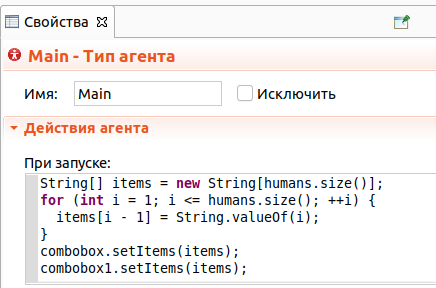
\includegraphics[scale=0.5]{agents3}
	\caption{Задание начальных значений выпадающих списков}
	\label{fig:agents3}
\end{figure}

Добавление связи между случайными агентами также осуществляется через кнопку. В данном алгоритме делается 100 раз попытка найти подходящую случайную вершину, то есть такую, которая не является текущей вершиной или вершиной-соседом с которым уже есть связь. Если за 100 итераций, такая вершина нашлась, то с ней возникает связь. (Рисунок \ref{fig:agents4})
\begin{figure}[h]
	\centering 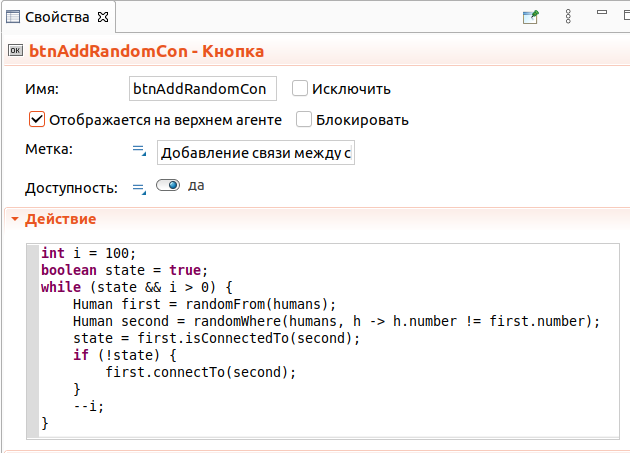
\includegraphics[scale=0.5]{agents4}
	\caption{Добавление связи между случайными агентами}
	\label{fig:agents4}
\end{figure}

Удаление связи между случайными агентами также реализовано по кнопке. В данном алгоритме делается 100 раз попытка найти подходящую случайную вершину, то есть такую, которая не является текущей вершиной или вершиной-соседом с которым нет связи. Если за 100 итераций, такая вершина нашлась, то связь с ней удаляется. (Рисунок \ref{fig:agents5})
\begin{figure}[h]
	\centering 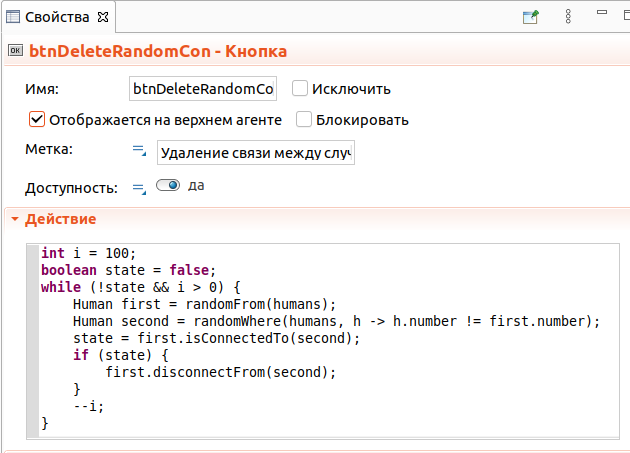
\includegraphics[scale=0.5]{agents5}
	\caption{Удаление связи между случайными агентами}
	\label{fig:agents5}
\end{figure}

Была реализована кнопка, по которой добавляется связь между двумя заданными вершинами. Вершины задаются через ComboBox. Если связь вершин является недопустимой, то ничего не происходит. (Рисунок \ref{fig:agents6})
\begin{figure}[h]
	\centering 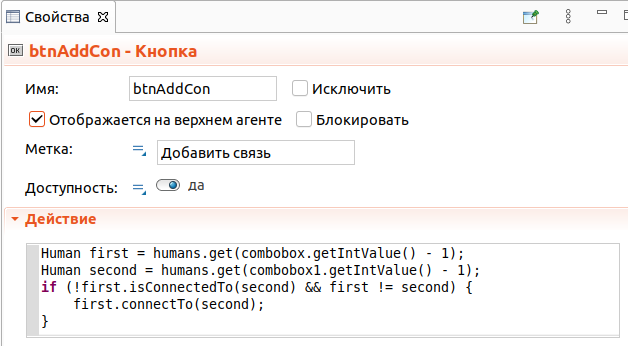
\includegraphics[scale=0.5]{agents6}
	\caption{Добавление связи между заданными вершинами}
	\label{fig:agents6}
\end{figure}

\newpage

По аналоги с добавлением связи между двумя заданными вершинами, была реализована кнопка удаление связи между двумя заданными вершинами. (Рисунок \ref{fig:agents7})
\begin{figure}[h]
	\centering 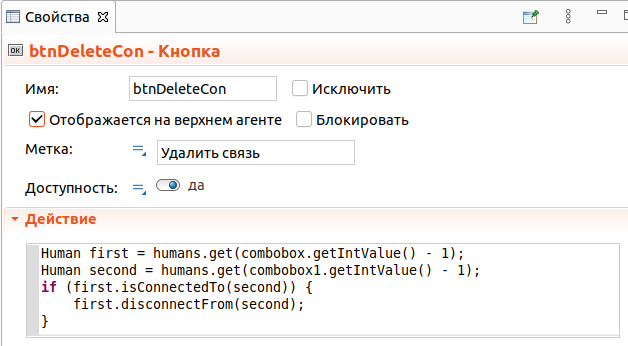
\includegraphics[scale=0.5]{agents7}
	\caption{Удаление связи между заданными вершинами}
	\label{fig:agents7}
\end{figure}

Далее в событии реализовано обновление агента с максимальным числом связей, он красился в красный, а всего его соседи красились в зелёный, остальные агенты в белый. (Рисунок \ref{fig:agents8})
\begin{figure}[h]
	\centering 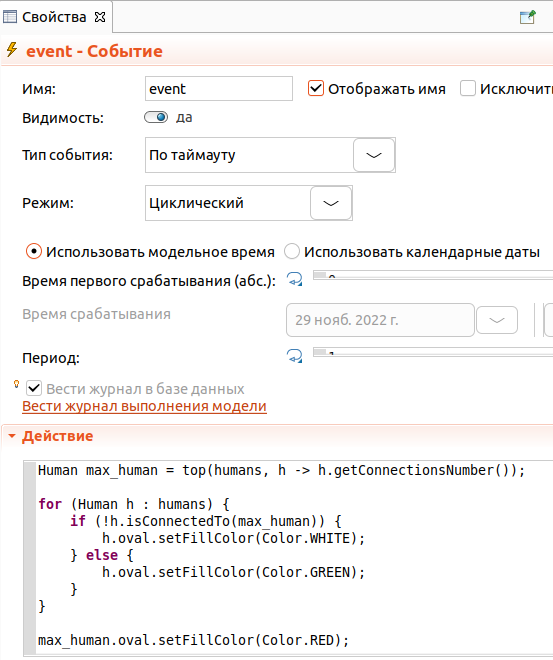
\includegraphics[scale=0.4]{agents8}
	\caption{Реализация события}
	\label{fig:agents8}
\end{figure}

\newpage

\begin{figure}[h]
	\centering 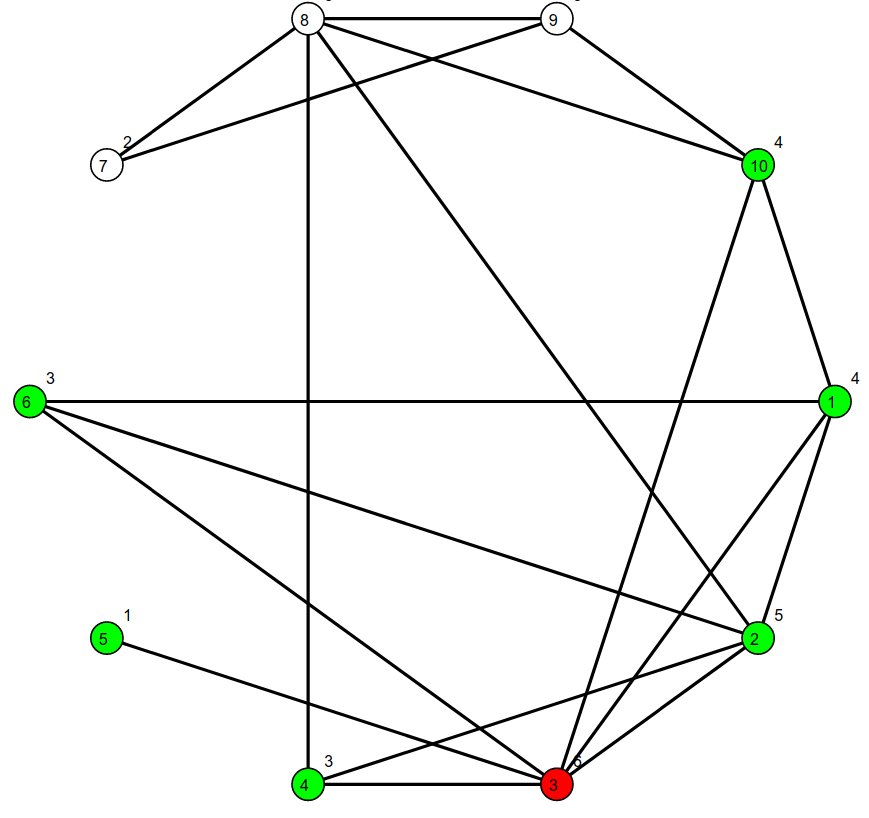
\includegraphics[scale=0.3]{agents9}
	\caption{Визуализация работы модели}
	\label{fig:agents9}
\end{figure}

Таким образом, в ходе реализации модели были разобраны основные инструменты для работы со связями агентов.